\chapter{Problem statement} \label{chap:problem-statement}

In this chapter, we first state an extension of the \ac{rcpsp} that we will use to model our studied problem.
Following this, we describe a constraint programming method used to find solutions to the problem.
Lastly, we present a formal framework for identifying bottlenecks, relaxing related constraints,
and obtaining improved solutions.

% ~~~~~~~~~~~~~~~~~~~~~~~~~~~~~~~~~~~~~~~~~~~~~~~~~~~~~~~~~~~~~~~~~~~~~~~~~~~~~~~~~~~~~~~~~~~~~~~~~~~~~~~~~~~
\section{Scheduling} \label{sec:problem-statement/scheduling}

We use the \Problem{} variant%
\footnote{$\alpha | \beta | \gamma$ three-field notation defined by \citet{Brucker1999}.}
of the \ac{rcpsp} to model the targeted real-world scheduling problem.
We extend the problem by introducing several new definitions to better model the addressed problem.
Furthermore, we introduce the notion of problem instances to help us distinguish between the original problem
and its modifications, as described in \cref{sec:problem-statement/relaxed-schedule}.
All following definitions and values are assumed to be in the integer domain.

\begin{defn}[Problem instance] \label{def:problem-instance}
A \emph{problem instance} $\Instance$ is defined as a 4-tuple $(\Jobs, \Precedences, \Resources, \horizon)$,
where
\begin{itemize}
    \item $\Jobs = \{1, \dots, n\}$ is a set of \emph{jobs},
    \item $\Precedences$ is a set of all \emph{precedences} constraints,
    \item $\Resources = \{1, \dots, m\}$ is a set of \emph{resources},
    \item $\horizon$ is the time horizon of the problem instance.
\end{itemize}
\end{defn}

\begin{figure}[p]
    \centering
    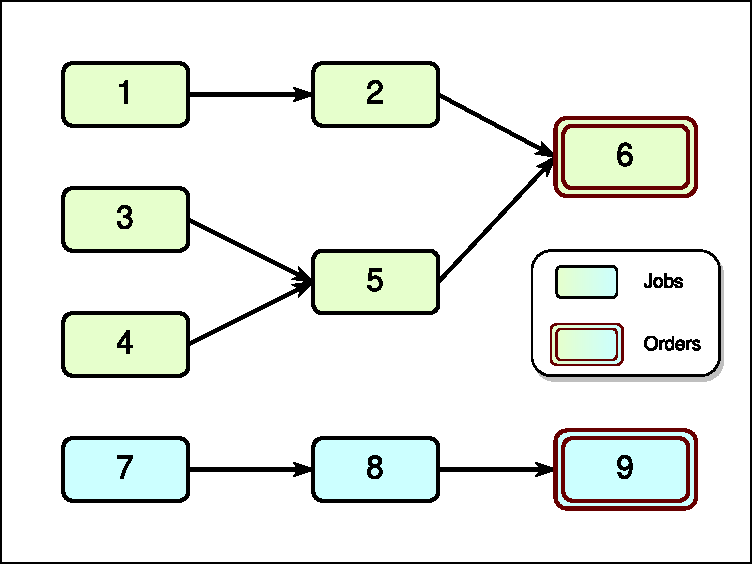
\includegraphics[width=0.6\textwidth]{img/Inforest.pdf}
    \caption{
        Example of a precedence graph.
        The inforest structure of the graph is demonstrated.
        Additionally, orders as the roots of the intrees are highlighted.}
    \label{fig:inforest}
\end{figure}

\begin{figure}[p]
    \centering
    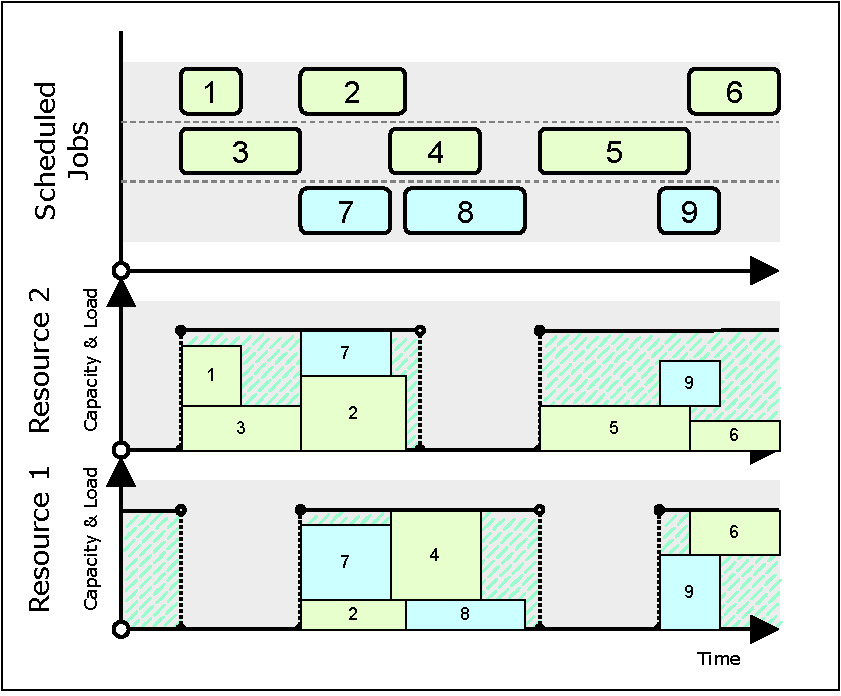
\includegraphics[width=0.999\textwidth]{img/Schedule.pdf}
    \caption{
        Example of a scheduled \ac{rcpsp} with time-variable resource capacities.
        The jobs with corresponding precedences from \cref{fig:inforest} are scheduled
        on two machines with partially overlapping working shifts.
        Job durations and capacity consumptions were chosen to illustrate the variability
        in resource utilization.
    }
    \label{fig:schedule}
\end{figure}

Each job $j \in \Jobs$ has a \emph{duration} $\duration{j}$,
describing the amount of time needed to process the job $j$.
\emph{Preemption} of jobs is not allowed in any form
--- the execution of a job cannot be interrupted after its start,
not even at the ends of working shifts (see variable resource capacities below).
Each job $j$ also has a \emph{due date} $\deadline{j}$,
stating a time horizon in which the job should be completed;
otherwise, it is considered \emph{tardy}.
Subsequently, each job $j$ also has a \emph{tardiness weight} $\tardinessweight{j}$
which defines a penalty accumulated for each unit of time the job is tardy.

Execution order of jobs is constrained with \emph{precedence constraints} $\Precedences$.
A precedence constraint between jobs $i$ and $j$,
denoted as $\precedence{i}{j}$ or $(i, j) \in \Precedences$,
states that the processing of job $j$ can start only after the processing of job $i$ was completed.

Interpreting jobs $\Jobs$ as vertices and precedences $\Precedences$ as edges between the jobs,
we define the \emph{precedence graph} $G = (\Jobs, \Precedences)$.
We assume the precedence graph to be an \emph{inforest}, in other words,
the precedences constrain the execution order of jobs in such a way that the resulting precedence graph
is always an inforest.
An~inforest is a directed acyclic graph where each vertex has at most one successor.
A connected subgraph of an inforest is an \emph{intree}.
See \cref{fig:inforest} for a precedence graph example.

Jobs are executed on \emph{resources} $\Resources$ --- machines with time-variant renewable \emph{capacities}.
The capacity of a resource $k$ during a time period $t \in \intinterval{1}{\horizon}$ is denoted as $\capacity{k}{t}$.
During their execution, jobs consume the capacities of resources.
For a job $j$, the per-period consumption of a resource $k$ is denoted as $\consumption{j}{k}$.
This describes how much of the resource's capacity is consumed each period during the job's execution.
Capacities are renewable, meaning that each time period the specified amount of capacity is available,
regardless of prior capacity consumptions.
The resource capacity functions $\capacity{k}{t}$ are assumed periodic with the same period of 24.
Moreover, the resource capacity function of the resource $k$ only takes the values
$0$ and $\shiftcapacity{k} \negmedspace>\! 0$.
This assumption, however, is only for the initial problem instance
--- resource capacity functions of modified instances, as described in \cref{sec:problem-statement/relaxed-schedule},
can be non-periodical and take arbitrary non-negative integer values.

The set of \emph{orders} $\Orders = \{ j \in \Jobs \mid \nexists i : \precedence{j}{i} \}$
is the set of roots of the precedence intrees,
i.e. the set of all jobs for which no precedence successor exists.
A job $j \in \Orders$ is called an \emph{order}.

We make a simple observation; due to the intree-structure,
each (weakly) connected component in the precedence graph contains exactly one order.
From this, we can say that each job is either an order
or is associated with a unique order within the same intree component.
This is demonstrated in \cref{fig:inforest}.

Having introduced orders, we can now specify the ranges of job deadlines and tardiness weights
based on whether a job belongs to the orders set $\Orders$:

$$
\deadline{j} = \begin{cases}
    a \in \Nzero  &\dots\;   \text{if $j \in \Orders$} \\
    +\infty       &\dots\;   \text{otherwise}
\end{cases}
\qquad
\tardinessweight{j} = \begin{cases}
    a \geq 0  &\dots\;   \text{if $j     \in \Orders$} \\
    0         &\dots\;   \text{otherwise}
\end{cases}
$$

% ~~~~~~~~~~~~~~~~~~~~~~~~~~~~~~~~~~~~~~~~~~~~~~~~~~~~~~~~~~~~~~~~~~~~~~~~~~~~~~~~~~~~~~~~~~~~~~~~~~~~~~~~~~~
\section{Constraint programming model} \label{sec:problem-statement/constraint-programming-model}

We formulate the above problem using a constraint programming model.
This provides us with a well-functioning framework
and allows us to use existing solvers for finding optimal solutions.
The model can be stated as:

\begin{align}
    \text{given}      && \multicolumn{4}{l}{$\Jobs = (1, \dots, n) ,\;%
                                             \Resources = (1, \dots, m) ,\;%
                                             \Precedences ,\;%
                                             $} \nonumber \\
                      && \multicolumn{4}{l}{$\duration{1}, \dots, \duration{n} \in \Nzero ,\;%
                                             \deadline{1}, \dots, \deadline{n} \in \intinterval{1}{\horizon} ,\;%
                                             \tardinessweight{1}, \dots, \tardinessweight{n} \in \Nzero ,\;%
                                             $} \nonumber \\
                      && \multicolumn{4}{l}{$\consumption{1}{1}, \dots, \consumption{n}{m} \in \Nzero ,\;%
                                             \capacityf{1}, \dots, \capacityf{m} : \intinterval{1}{\horizon} \to \Nzero %
                                             $} \nonumber \\
    \text{find}       && \multicolumn{4}{l}{$\Schedule = (\jobstart{1}, \dots, \jobstart{n}) \in \N^n$} \nonumber \\
    \text{minimizing} && \sum_{j \in \Jobs} \tardinessweight{j} \tardiness{j}
                      &
                      &&
                      \label{csp:objective} \\
    \text{subject to} && \jobend{i}
                      & \leq \jobstart{j}
                      && \forall \precedence{i}{j} \in \Precedences
                      \label{csp:precedences} \\
                      && \sum_{j \in \Jobs} \modelConsumption{j}{k}{t}
                      & \leq \capacity{k}{t}
                      && \forall t \in \intinterval{1}{\horizon} \; \forall k \in \Resources
                      \label{csp:capacities} \\
    \text{where}      && \multicolumn{4}{l}{$\Completions = (\jobstart{1} + \duration{1}, \dots, \jobstart{n} + \duration{n}) ,\;%
                                             \tardiness{j} = \max(0, \jobend{j} - \deadline{j}) ,\;%
                                             $} \nonumber \\
                      && \multicolumn{4}{l}{$\modelConsumption{j}{k}{t} \defeq \begin{cases}
                                                 \consumption{j}{k} & \text{if $\jobstart{j} \leq t < \jobend{j}$} \\
                                                 0                  & \text{otherwise}
                                                 \end{cases}
                                             $} \nonumber
\end{align}

Inequalities \eqref{csp:precedences} formulate the precedence constraints --- start and finish times of jobs
are according to all the precedences.
Inequalities \eqref{csp:capacities} formulate the resource capacity constraints --- in every time period
the combined consumption of jobs scheduled during the period cannot exceed any of the resource's capacities.
Expression \eqref{csp:objective} is the optimization minimization objective --- the weighted tardiness of jobs.

We assume we have a solver capable of solving \eqref{csp:objective}--\eqref{csp:capacities} in reasonable time
through the use of constraint programming.

In the following sections, we will consider the stated constraints as potential bottlenecks
and how to relax specific constraints identified as bottlenecks.

% ~~~~~~~~~~~~~~~~~~~~~~~~~~~~~~~~~~~~~~~~~~~~~~~~~~~~~~~~~~~~~~~~~~~~~~~~~~~~~~~~~~~~~~~~~~~~~~~~~~~~~~~~~~~
\section{Bottlenecks} \label{sec:problem-statement/bottlenecks}

% -----------------------------------------------------------------------------------------------------------
\subsection{Definition} \label{subsec:problem-statement/bottlenecks/definition}

Our goal will be to find bottlenecks in the problem, specifically in the obtained schedule
--- the solution to the constraint programming model defined in \cref{sec:problem-statement/constraint-programming-model}.
First, we state a general definition of an execution-level bottleneck:

\begin{defn}[\acf{ebm} \citep{Wang2016}] \label{def:bottleneck}
    \emph{\ac{ebm}} is a machine that dominates the scheduling performance in the strongest manner
    at the execution level of production systems.
\end{defn}

The execution level of a production system stated here refers to finding bottlenecks
specific to the given problem instance and the obtained solution to that instance.
This is consistent with our goal of finding bottlenecks in the particular problem instances and their solutions,
and improving the system performance only with respect to the currently presented problem.
In contrast, we will not be interested in bottlenecks of the whole system
nor in generally improving the performance of the system regardless of the problem instance.
Having made the distinction, we will now discuss our interpretation of the definition suited to our problem.

Instead of identifying just a single machine as a bottleneck
or listing all the machines in the order of their scheduling impact,
we will focus on identifying specific time periods on specific machines as schedule bottlenecks.
This allows us to relax only the specific constraints related to the identified time periods,
resulting in localized modifications with minimal costs.

% -----------------------------------------------------------------------------------------------------------
\subsection{Constraints relaxation} \label{subsec:problem-statement/bottlenecks/constraints-relaxation}

When deciding which constraints to relax,
we have two constraints to consider: precedence constraints \eqref{csp:precedences}
and resource capacity constraints \eqref{csp:capacities}.
We will discuss individual segments that form the constraints,
considering their possible relaxation.

\begin{enumerate}[label=(\roman*)]
    \item \emph{Job precedences}
    Job precedence constraints are inherent to the problem ---
    --- jobs cannot start until all their predecessors have finished executing.
    We cannot remove individual precedences as a relaxation,
    as precedences model the technological requirements of the production system.
    We could imagine that scheduling jobs might require preparations,
    which do not necessarily require the presence of the product about to be processed.
    Those preparations could therefore be allowed to start even before the predecessor jobs finish executing,
    which would introduce slack in the constraints%
    \footnote{
    Scheduling with so-called \emph{setup times} is a broadly studied subject in the literature.
    See the survey of \citet{Hartmann2010} where the extension of setup times is described
    and various examples of approaches to the problem are given.
    }.
    However, we can assume that those preparations are completed before the start,
    or we can assume no preparation time at all.

    \item \emph{Cumulative consumption}
    The cumulative consumption is dependent on the constructed schedule and the given problem instance.
    Each job contributes to the cumulative consumption during the time periods it is scheduled.
    As part of the problem definition, we cannot omit this contribution,
    nor can it be shortened, as job durations $\duration{j}$ are fixed.
    Equally, job resource consumptions $\consumption{j}{k}$ influence the cumulative value,
    but again, due to the nature of our problem,
    we cannot modify resource consumptions as those are inherent to the problem
    and the corresponding real-life execution and operation requirements.

    \item \emph{Resource capacities}
    Available capacities of resources can be modified with reasonable correspondence
    to modifications of the real-life problem.
    More specifically, the capacity of a resource during a time period can be increased or decreased.
    Increasing the capacity of a resource during specific time periods could correspond to increasing
    the number of workers operating the resource machine,
    assuming that increasing the number of operating workers increases the total processing capacity.
    While sole reduction of capacities would not relax the constraints,
    decreasing the capacity of one resource by a specific amount
    while increasing the capacity of another resource
    by the same amount could tighten the constraints on the former resource
    but relax the constraints on the latter.
    This decreasing of the capacity of one resource
    while increasing the capacity of another by the same amount
    could correspond to migrating workers between the resource machines,
    assuming that migrations of operating workers are possible.
\end{enumerate}

We can conclude that the precedence constraints \eqref{csp:precedences} cannot be relaxed.
On the other hand, the resource capacity constraints \eqref{csp:capacities}
can be relaxed by modifying the capacities of resources.
As discussed,
these modifications can be achieved through capacity additions or migrations,
both of which have corresponding realizations in real-world production systems.

% -----------------------------------------------------------------------------------------------------------
\subsection{Resource capacity modifications} \label{subsec:problem-statement/bottlenecks/resource-capacity-modifications}

We will consider \emph{capacity additions} and \emph{capacity migrations} as the possible relaxations
of scheduling constraints, namely of the constraints \eqref{csp:capacities}.
Additions are executed by increasing the capacity of a selected resource
by a specified amount over a specified time interval.
Migrations are executed by decreasing the capacity of a selected source resource
by a specified amount over a specified time interval
and increasing the capacity of a selected target resource
by the specified amount over the same time interval.
An illustrative example of a capacity addition and a capacity migration is shown in \cref{fig:CapacityChanges}.

We consider migrations only between resources, limited to the same time interval.
We do not allow migrations in time ---
reducing the capacity of the source resource during a time interval
and then increasing the capacity of a target resource during a different interval.
Such migrations could correspond to migrating resource materials between resources.
In such cases, the change in time would correspond to the migrated material
being processed at a different time on a different machine.
However, we consider production systems with workers and machine operators as main resource capacities.
Considering this, migrating capacities in time would not have practical realizations,
as the workers migrated from one resource during one time period
would likely still be assigned to that that resource during a different time period.

\begin{figure}
    \centering
    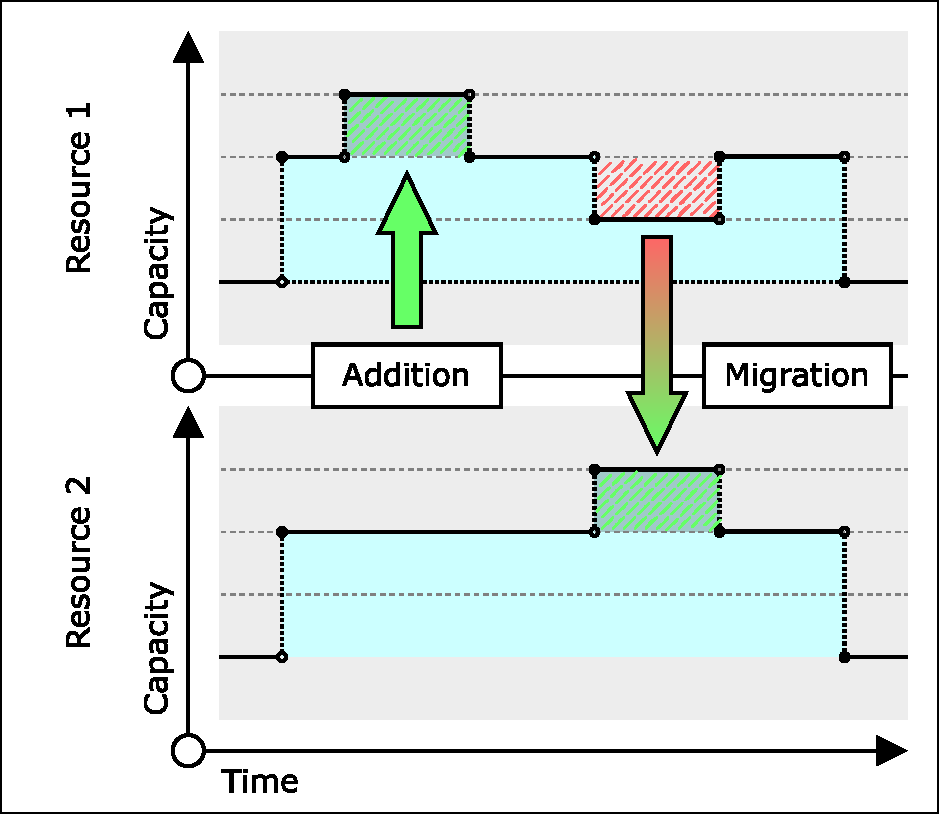
\includegraphics[width=0.7\textwidth]{img/Capacities-Changes.pdf}
    \caption{Diagram of possible capacity changes}
    \label{fig:CapacityChanges}
\end{figure}

We associate a capacity addition with the 4-tuple $\addition{k}{s}{e}{c}$, where
$k$ is the resource whose capacity is increased,
$s$ and $e$ form the time interval $\intinterval{s}{e}$ over which the addition is executed, and
$c$ is the added capacity.
Analogously, we associate a capacity migration
with the 5-tuple $\migration{k_{\text{from}}}{k_{\text{to}}}{s}{e}{c}$, where
$k_{\text{from}}$ is the source resource whose capacity is lowered,
$k_{\text{to}}$ is the target resource whose capacity is increased,
$s$ and $e$ form the time interval $\intinterval{s}{e}$ over which the migration is executed, and
$c$ is the migrated capacity.
For a modified instance $\Instance^*$, the sets of all migrations and additions are denoted as
$\Migrations^{\Instance^*}$ and $\Additions^{\Instance^*}$, respectively.

In a real-world production system,
migrating capacities is generally more cost-effective than adding new capacities.
For example, reassigning workers from an underutilized machine to a bottleneck machine
is typically less expensive than extending workers' shifts into overtime
or planning an entirely new and irregular shift.
Therefore, capacity migrations are usually preferred.
However, if the required capacity changes cannot be achieved through capacity migrations,
capacity additions can be utilized.

% ~~~~~~~~~~~~~~~~~~~~~~~~~~~~~~~~~~~~~~~~~~~~~~~~~~~~~~~~~~~~~~~~~~~~~~~~~~~~~~~~~~~~~~~~~~~~~~~~~~~~~~~~~~~
\section{Relaxed schedule} \label{sec:problem-statement/relaxed-schedule}

In the rest of this chapter, we define a general procedure for solving the presented problem,
identifying bottlenecks and relaxing corresponding constraints by modifying the initial problem,
solving the modified problem,
and evaluating whether the modified solution reached a desired improvement.
More precisely:

\begin{enumerate}
    \item Suppose we obtained an optimal solution $\Schedule$ to the problem instance $\Instance$.

    \item We select the target order $\targetOrder \in \Orders$ for which we want to improve the tardiness.
        We consider improvement to be any non-zero decrease in the objective function with respect to the
        selected order $\targetOrder$ and its tardiness $\tardiness{\targetOrder}$.

    \item We identify bottlenecks in the solution $\Schedule$ of the instance $\Instance$.

    \item Based on the identified bottlenecks, corresponding constraints are relaxed via
        capacity additions and capacity migrations.
        Those capacity changes are captured by modified resource capacity functions
        $\capacityf{1}^*, \ldots, \capacityf{m}^*$
        corresponding to a modified problem instance $\Instance^*$.

    \item We obtain a solution $\Schedule^*$ to the modified problem instance $\Instance^*$.

    \item Finally, any desired evaluations can be made on the modified solution $\Schedule^*$,
        alongside comparisons to the original solution $\Schedule$.
\end{enumerate}
